\subsection{Ionic mit Cordova beziehungsweise Capacitor}
\label{sec:Frameworks_Ionic}

Das Ionic-Framework ist selbst kein Cross-Plattform Framework, sondern ein UI-Toolkit \cite{Ionic_Docs}.
Damit unterstützt Ionic nur die Erstellung plattformübergreifender Oberflächen.
Wie \autoref{fig:ionic_architecture} zeigt, wird Ionic in Verbindung mit Apache Cordova oder Capacitor verwendet.
Ionic lässt sich allerdings auch in reinen Webanwendungen nutzen \cite{Ionic_Docs}.
\begin{figure}[h]
    \centering
    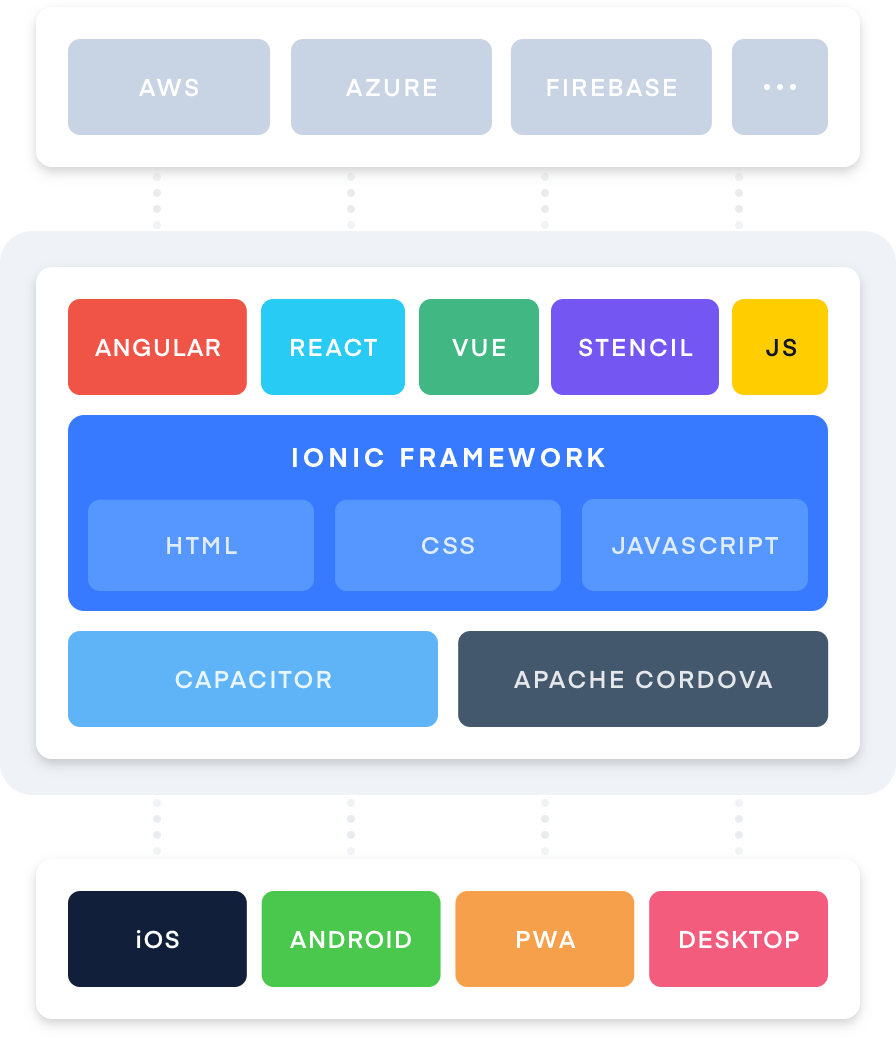
\includegraphics[clip, trim=0cm 0cm 0 8cm,height=8cm]{ionic_architecture.png}
    \caption{Architektur des Ionic-Frameworks \cite{Ionic_Architektur}}
    \label{fig:ionic_architecture}
\end{figure}


Ionic stellt \ac{UI}-Komponenten zur Verfügung, die plattformübergreifend genutzt werden können und automatisch dem Stil der jeweiligen Plattform angepasst werden.
Zur weiteren Vereinfachung unterstützt Ionic die Verwendung der beliebten Frontend-Frameworks und Bibliotheken Angular, React und Vue.js, welche das Erstellen von Oberflächen weiter vereinfachen \cite{Ionic_Docs, Ionic_EvaluationGuide}.
Außerdem bietet Ionic eine Reihe von Zusatzleistun für zahlende Kunden an, wie beispielsweise persönliche Beratung und Support und proprietäre Plugins für Funktionen, die nicht über Open-Source Plugins abgedeckt werden können \cite{Ionic_EvaluationGuide}.



Die beiden unterstützen Cross-Plattform Frameworks Cordova und Capacitor sind sich im Allgemeinen sehr ähnlich.
Beide ermöglichen es, Webanwendungen in native Anwendungen einzubetten und über ein Plugin-System auf native \acp{API} zuzugreifen \cite{Ionic_Cordova_vs_Capacitor}.


Apache Cordova ist das deutlich ältere Framework und wird als Open-Source-Projekt von der Apache Software Foundation verwaltet.
Die Open-Source Version des ursprünglich kommerziellen Frameworks \textit{PhoneGap} wurde 2011 an die Apache Software Foundation übergeben \cite{Steyer_Cordova}.
Seit 2020 wird die kommerzielle Version des Frameworks im Vergleich zur Open-Source Variante nicht mehr weiter entwickelt \cite{Adobe_PhoneGap_EOL}.


Zur Unterstützung mehrerer Plattformen verwendet Cordova den Ansatz einer Hybrid Web App.
Jede Web-App, welche mit \ac{HTML}, \ac{CSS} und JavaScript entwickelt wurde, lässt sich mit Cordova als native Anwendung verpacken.
Mit Cordova sind Web-Apps, ohne den Umweg über einen Browser, direkt auf der Plattform ausführbar und lassen sich über die App-Stores der jeweiligen Plattformen verbreiten.
Dazu verwendet Cordova eine Wrapper-Anwendung, welche die eigentliche Web-App in einer WebView ausführt.
\autoref{fig:cordova_architecture} zeigt die Architektur, die sich durch diese Einbettung der Web-App ergibt.
\begin{figure}[h]
    \centering
    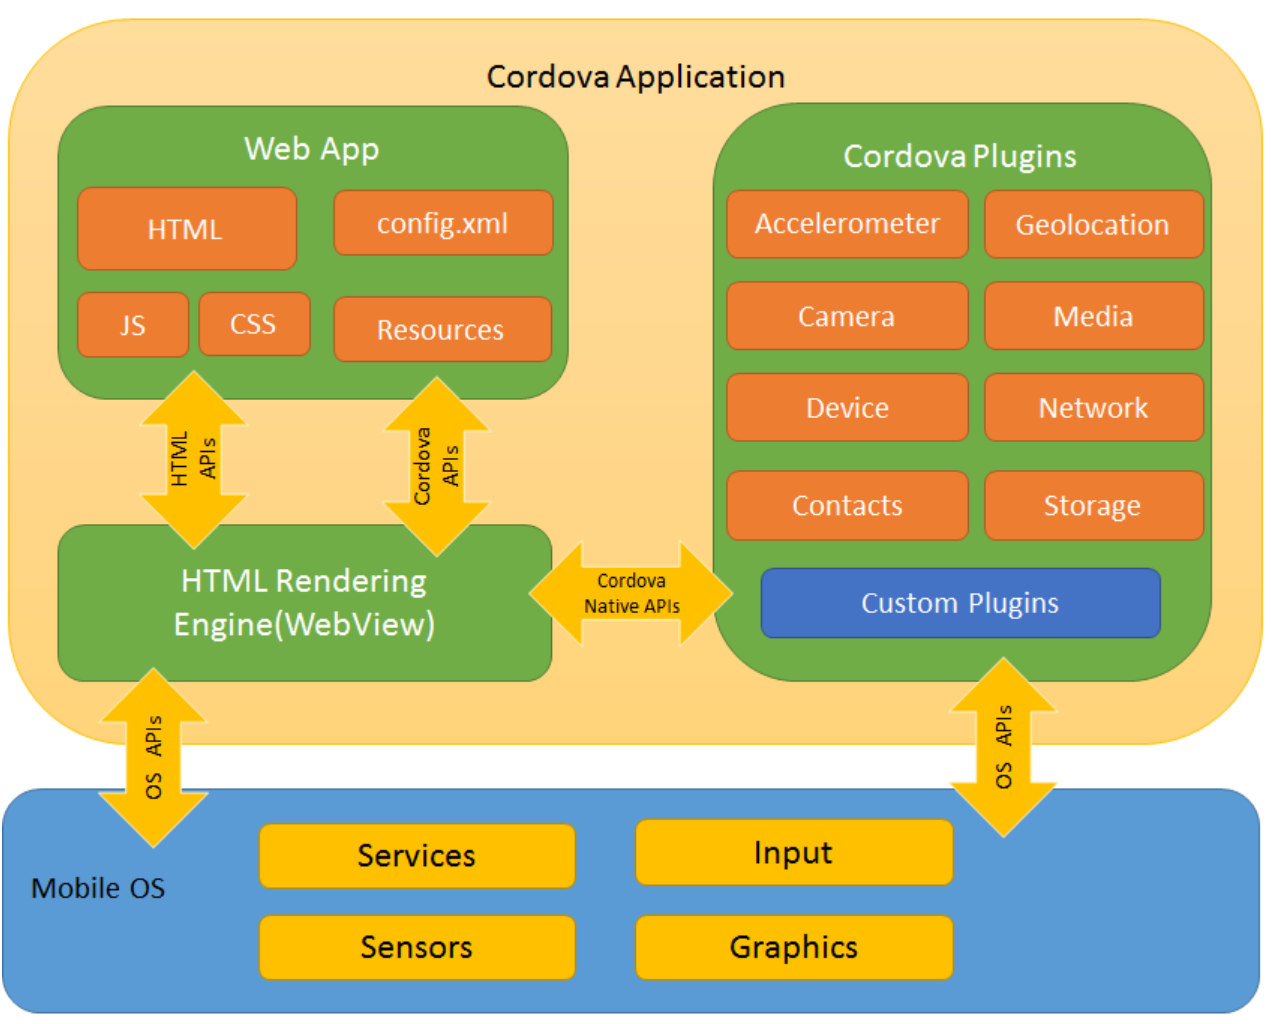
\includegraphics[height=10cm]{cordova_architecture.png}
    \caption{Überblick über die Architektur einer Cordova-Anwendung \cite{Cordova_Overview}.}
    \label{fig:cordova_architecture}
\end{figure}
Die WebView ist ein eingebetteter Webbrowser, der vom Betriebssystem bereitgestellt wird \cite{Steyer_Cordova}.
Die Web-App kann Cordova-\acp{API} nutzen, um über die WebView auf Plugins zuzugreifen.
Diese Plugins bestehen aus einer JavaScript-Schnittstelle und einer plattformspezifischen nativen Implementierung \cite{Steyer_Cordova,Heitkoetter_CrossPlatform_Comparison}.
Für häufig verwendete Gerätefunktionen und \acp{API} sind entweder offizielle Plugins der Apache Software Foundation oder sonstige Open-Source Plugins verfügbar.
Werden die benötigten Funktionen nicht von verfügbaren Plugins bereitgestellt, können eigene Plugins für die jeweiligen Plattformen entwickelt werden \cite{Cordova_Overview}.
Damit sind alle Gerätefunktionen mit gewissem Aufwand nutzbar \cite{Steyer_Cordova}.
Werden Funktionen benötigt, für die keine Plugins verfügbar sind, steigt der Entwicklungsaufwand durch die Entwicklung eigener Plugins für jede zu unterstützende Plattform deutlich an.
Damit der große Vorteil der Cross-Plattform Entwicklung erhalten bleibt, sollten so wenige spezifische Plugins entwickelt werden müssen wie möglich.

Capacitor wurde 2018 von Ionic als modernere Alternative zu Cordova vorgestellt und führt Web-Apps ebenfalls in einer WebView aus.
Um den Umstieg von Cordova auf Capacitor zu erleichtern, können alle Cordova-Plugins direkt in Capacitor-Projekte eingebunden werden \cite{Liebel_Cordova_Capacitor}.
Zudem erlaubt Capacitor durch ein geändertes Build-Konzept eine einfachere Integration von nativem Code, ohne den Einsatz von Plugins \cite{Ionic_Cordova_vs_Capacitor}.
In Cordova-Projekten werden die nativen Projekte für die Wrapper-Anwendungen beim Build erzeugt und der Web-Code in diese eingebettet.
Bei Capacitor-Projekten werden die nativen Projekte für die Wrapper-Anwendungen stattdessen bereits zu Beginn erstellt und sollen in die Versionsverwaltung aufgenommen werden.
Dadurch kann nativer Code direkt in die jeweiligen nativen Projekte integriert werden und wird nicht beim nächsten Build überschrieben \cite{Liebel_Cordova_Capacitor}.


Die Performance von Ionic und Cordova-basierten Anwendungen gilt allgemein als niedrig.
Bei reinen Cordova-Anwendungen wird zusätzlich die Konsistenz der \ac{UI} häufig kritisiert \cite{Steyer_Cordova}.
Beides ist auf die Einbettung von Web-Apps in native Wrapper-Anwendungen zurückzuführen.
Durch die Interpretation von JavaScript-Code innerhalb der WebView und den aufwändigen Zugriff auf native Funktionen über das komplexe Plugin-System, liegt die Performance von Cordova-Anwendungen deutlich unter der von nativen Anwendungen und häufig auch unter der von anderen Frameworks \cite{Rieger_CrossPlatform_EvaluationFramework,Biorn-Hansen_PerformanceOverhead_CrossPlatform}.


Capacitor ist trotz geringerer Verbreitung deutlich beliebter als Cordova \cite{Stackoverflow_2022,Appfigures_TopSDKs}.
Von allen Entwicklern, die bereits mit Capacitor gearbeitet haben, geben 62,35 \% an, das Framework auch weiterhin einsetzen zu wollen.
Nur 28,85 \% wollen Cordova weiter verwenden.
Damit schneidet Cordova von allen betrachteten Cross-Plattform Frameworks am schlechtesten ab.